\chapter{Практический раздел}

\section{EBNF грамматика выражений логики предикатов}

Ниже приведена грамматика выражений логики предикатов, реализованная в данной лабораторной работе.

\begin{verbatim}
<expr>       ::= <equ>
<equ>        ::= <disj> <eq-sign> <equ>
<disj>       ::= <impl> '+' <disj>
<impl>       ::= <conj> '->' <impl>
<conj>       ::= <quant> '&' <conj>
<quant>      ::= [ <quant-list> ] <term>
<term>       ::= '(' <expr> ')' | <neg> | <atom>
<neg>        ::= '~' <quant>
<equ-sign>   ::= '==' | '=' | '<=>' | '<->'
<atom>       ::= IDENT [ '(' <arg-list> ')' ]
<arg-list>   ::= <arg> [ ',' <arg-list> ]
<arg>        ::= IDENT [ '(' <arg-list> ')' ]
<quant-list> ::= <quantifier> [ <quant-list> ]
<quantifier> ::= '\forall' '(' <var-decl> ')'
               | '\exists' '(' <var-decl> ')'
<var-decl>   ::= IDENT [ ',' <var-decl> ]    
\end{verbatim}

В качестве примера, формула
\begin{equation*}
    \forall x \forall y (\neg P(x, f(C)) \rightarrow \exists z (Q(x, z) \& P(g(x), y)))
\end{equation*}
по правилам представленной грамматики записывается в следующем виде
\begin{verbatim}
\forall(x, y) (~P(x, f(C)) -> \exists(z) (Q(x, z) & P(g(x), y)))
\end{verbatim}

\clearpage

\section{Алгоритм унификации двух атомов}

Схема алгоритма унификации двух атомов представлена на рисунке \ref{fig:unify-atom}.

\begin{figure}[h!]
    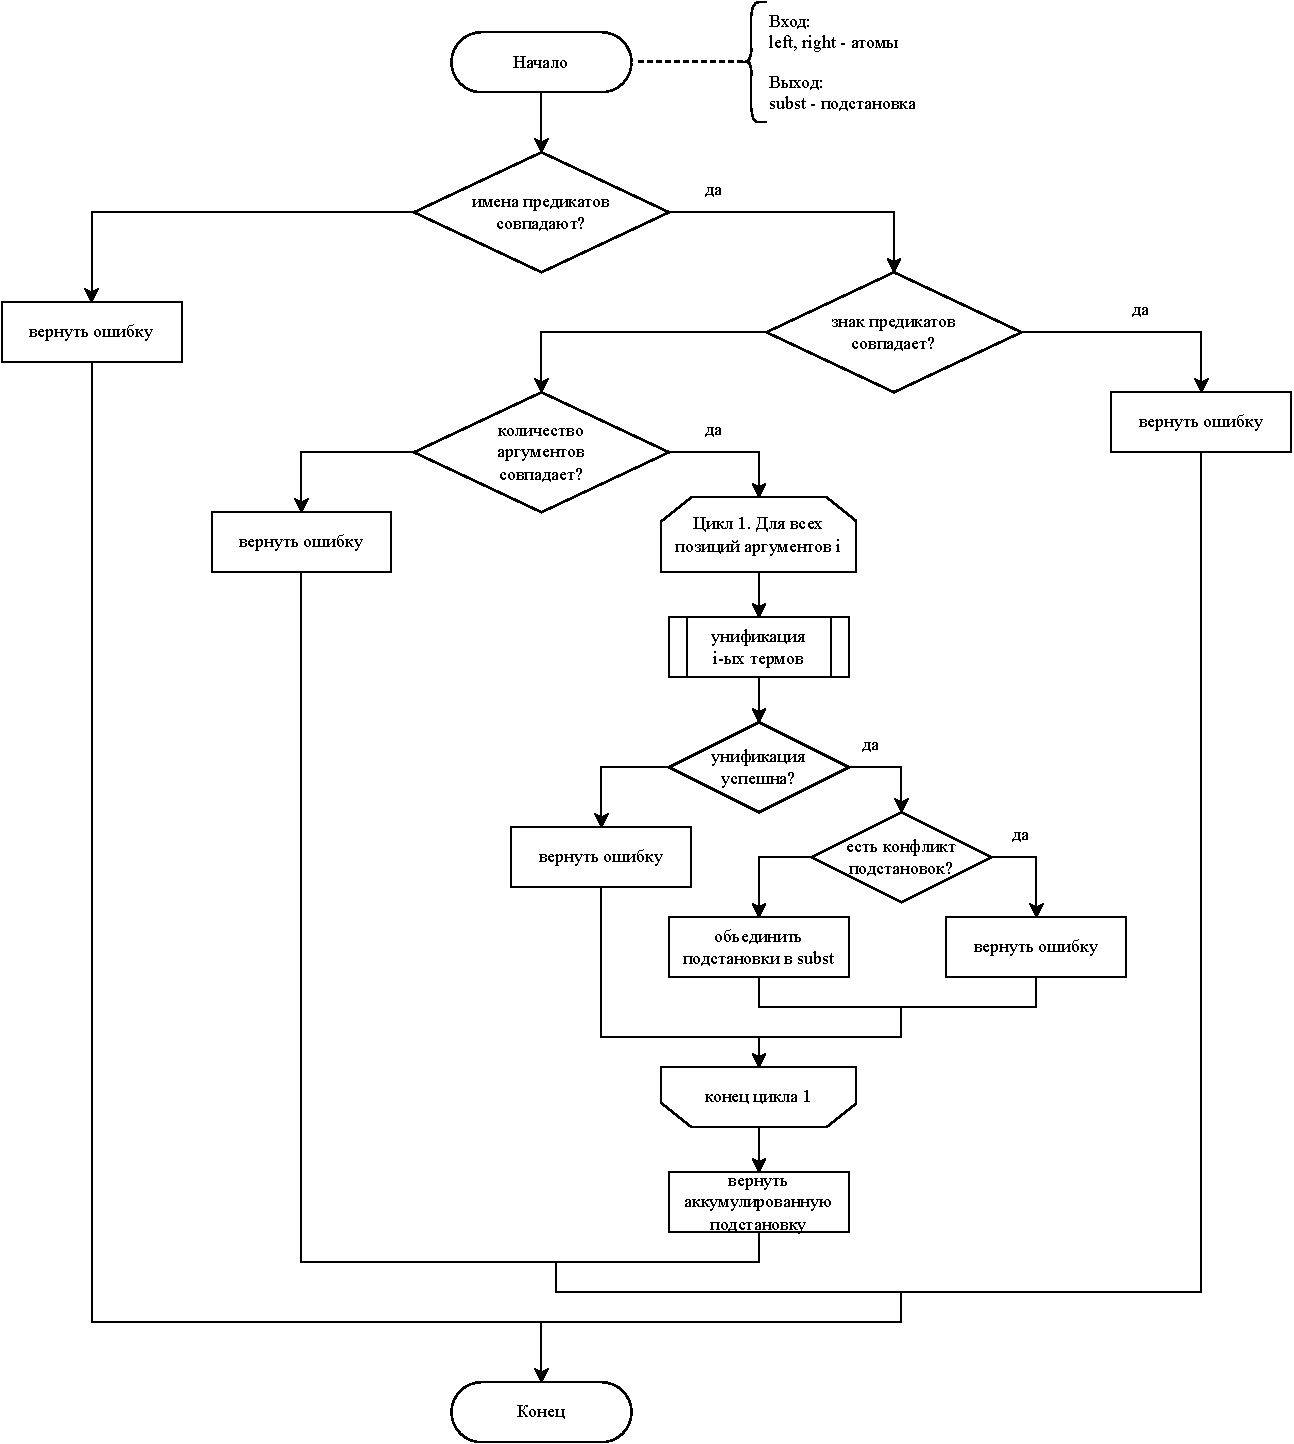
\includegraphics[width=\linewidth]{unify-atom.pdf}
    \caption{Схема алгоритма унификации двух атомов}
    \label{fig:unify-atom}
\end{figure}

\textbf{Определение конфликта подстановок}. Так как в процессе унификации распространение значения переменных не используется, необходимо отслеживать непротиворечивость генерируемых подстановок. \textbf{Конфликт двух подстановок} определяется выполнением хотя бы одного условия:

\begin{enumerate}
    \item имеются две переменные в этих подстановках, имеющие одинаковые имена, но связанные с разными (неунифицируемыми) значениями;
    \item существует список связанных, но не означенных переменных в одной подстановке, для которой найдутся две переменные, связанные с разными значениями в другой подстановке.
\end{enumerate}

Назовем множество имен $A$ \textbf{непротиворечивым на подстановке} $B$, если все имена из $A$ либо не связаны со значениями в $B$, либо связаны с одним и тем же значением в $B$.

\textbf{Объединение подстановок}. Объединение подстановок (назовем их $A$ и $B$) происходит следующим образом:

\begin{enumerate}
    \item если подстановка $A$ пуста, то вернуть $B$;
    \item если подстановка $B$ пуста, то вернуть $A$;
    \item создать новую подстановку $C := A$;
    \item для всех пар [имя переменной $v$, значение $t$] из списка связанных значений подстановки $B$:
    \begin{enumerate}
        \item если имя переменной $v$ связано со значением $u$ в подстановке $C$ и $t \ne u$:
        \begin{enumerate}
            \item запустить процесс унификации для $t$ и $u$;
            \item если унификация неуспешна --- вернуть ошибку;
            \item иначе применить полученную подстановку к значению $u$;
            \item связать имя переменной $v$ с новым значением $u$;
        \end{enumerate}
        \item иначе связать имя переменной $v$ со значением $t$ в $C$;
    \end{enumerate}
    \item для всех множеств имен связанных переменных $S$ в подстановке $B$:
    \begin{enumerate}
        \item для всех множеств имен связанных переменных $T$ в подстановке $C$:
        \begin{enumerate}
            \item если $S \cap T \ne \emptyset$, то переход на следующую итерацию цикла;
            \item расширить множество имен переменных $T \leftarrow S \cup T$;
            \item проверить \textbf{непротиворечивость множества имен} $T$ в $C$;
            \item если полученное множество противоречиво --- вернуть ошибку;
            \item иначе --- завершить цикл;
        \end{enumerate}
        \item если на предыдущем цикле не было расширено ни одно множество, то проверить на непротиворечивость множество имен $S$ в $C$;
        \item если множество противоречиво -- вернуть ошибку; 
        \item иначе --- добавить множество имен связанных переменных $S$ в $C$; 
    \end{enumerate}
    \item для для всех пар [имя переменной $v$, значение $t$] из списка связанных значений подстановки $C$:
    \begin{enumerate}
        \item \textbf{разрешить рекурсию} для значения $t$ в $C$;
    \end{enumerate}
    \item вернуть подстановку $C$.
\end{enumerate}

\textbf{Алгоритм разрешения рекурсии} подставляет значения переменных в функциональные символы, которые были связаны с другими переменными во время слияния подстановок. Рассмотрим пример слияния неконфликтующих подстановок $\{x = f(y)\}$ и $\{y = g(x)\}$. Схема данного процесса изображена на рисунке \ref{fig:func-rec}. Цель данного алгоритма --- избавиться от ссылок на переменные связанные со значениями в данной подстановке из функциональных символов присутствующих в этой подстановке.

\begin{figure}[h!]
    \centering
    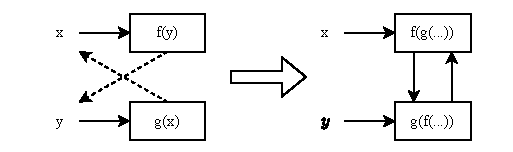
\includegraphics[width=0.7\linewidth]{func-recursion.pdf}
    \caption{Схема разрешения рекурсии}
    \label{fig:func-rec}
\end{figure}

Шаги алгоритма разрешения рекурсии для значения $t$ подстановки $C$:

\begin{enumerate}
    \item если $t$ --- не функциональный символ, завершить процедуру;
    \item для всех агрументов функционального символа $t$:
    \begin{enumerate}
        \item если аргумент --- переменная, то заменить ее результатом применения подстановки $C$ к этой переменной;
        \item иначе если аргумент --- функциональный символ, то \textbf{разрешить рекурсию} для этого функционального символа.
    \end{enumerate}
\end{enumerate}

\clearpage

\section{Алгоритм унификации двух термов}

Схема алгоритма унификации двух термов представлена на рисунке \ref{fig:unify-term}.

\begin{figure}[h!]
    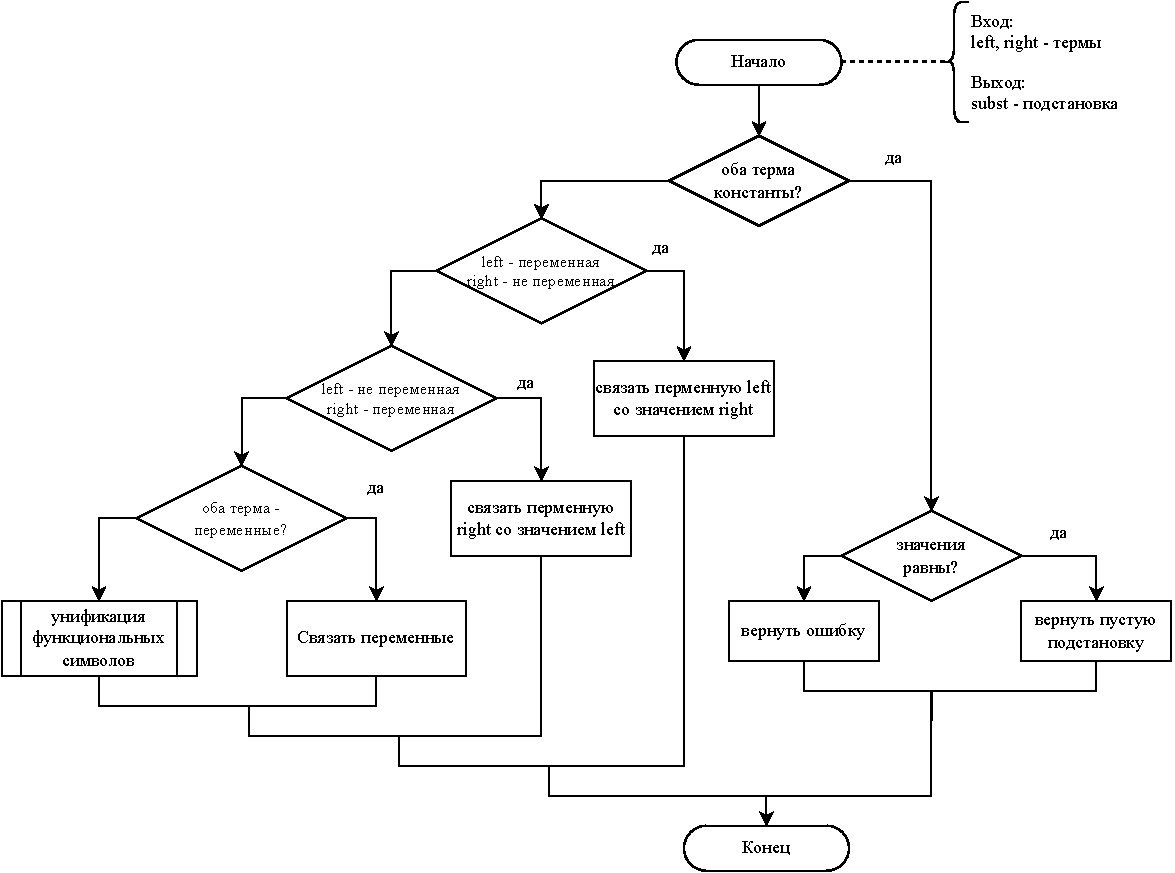
\includegraphics[width=\linewidth]{unify-term.pdf}
    \caption{Схема алгоритма унификации двух термов}
    \label{fig:unify-term}
\end{figure}

Унификация функциональных символов производится рекурсивно для аргументов функции после проверки соответствия имен функций и количества аргументов согласно представленному алгоритму. После чего осуществляется композиция подстановок. В случае возникновения конфликтов, определяется, что исходные функциональные символы не унифицируемы.

Так как составленная грамматика выражений логики предикатов первого порядка не допускает записи рекурсивных функциональных символов, то и унифицировать их не нужно.

\section{Алгоритм поска резольвенты для двух дизъюнктов}

Алгоритм поиска резольвенты для двух дизъюнктов заключается в простом переборе всех возможных пар атомов из исходных дизъюнктов и попытке их унификации. Если унификация успешна, то конструируется новый дизъюнкт, состоящий из всех атомов исходных дизъюнктов за исключением унифицированной пары. После составления дизъюнкта к нему применяется полученная на этапе унификации подстановка и результат возвращается из процедуры резолюции двух дизъюнктов.

\textbf{Алгоритм применения подстановки к дизъюнкту} заключаеся в последовательном применении подстановки ко всем атомам этого дизъюнкта.

\textbf{Алгоритм применения подстановки к атому} заключается в последовательном применении подстановки ко всем аргументам этого атома (если они есть).

\textbf{Алгоритм применения подстановки к терму} на входе и на выходе имеет терм. Шаги алгоритма:

\begin{enumerate}
    \item если терм --- константа, то вернуть этот же терм;
    \item если терм --- переменная:
    \begin{enumerate}
        \item если переменная есть в списке означенных переменных, то вернуть значение, соответствующее этой переменной;
        \item иначе для всех списков связанных переменных проверить, если имя терма принадлежит текущему списку связанных переменных, то вернуть первое имя из этого списка;
        \item иначе вернуть этот же терм;
    \end{enumerate}
    \item иначе если у терма нет аргументов, то вернуть этот терм;
    \item иначе применить подстановку ко всем аргументам и вернуть новый функциональный символ с полученным списком аргументов.
\end{enumerate}

\section{Алгоритм резолюции}

Алгоритм резолюции состоит из полного последовательного перебора всех возможных пар дизъюнктов и поиска для них резольвенты. В случае успешного нахождения резольвента добавляется в конец списка дизъюнктов и процесс продолжается. Условием останова является получение пустой резольвенты, либо полный перебор с учетом вновь добавленных резольвент, либо достижение максимального количества итераций.

\section{Диаграмма классов}

\begin{figure}[h!]
    \centering
    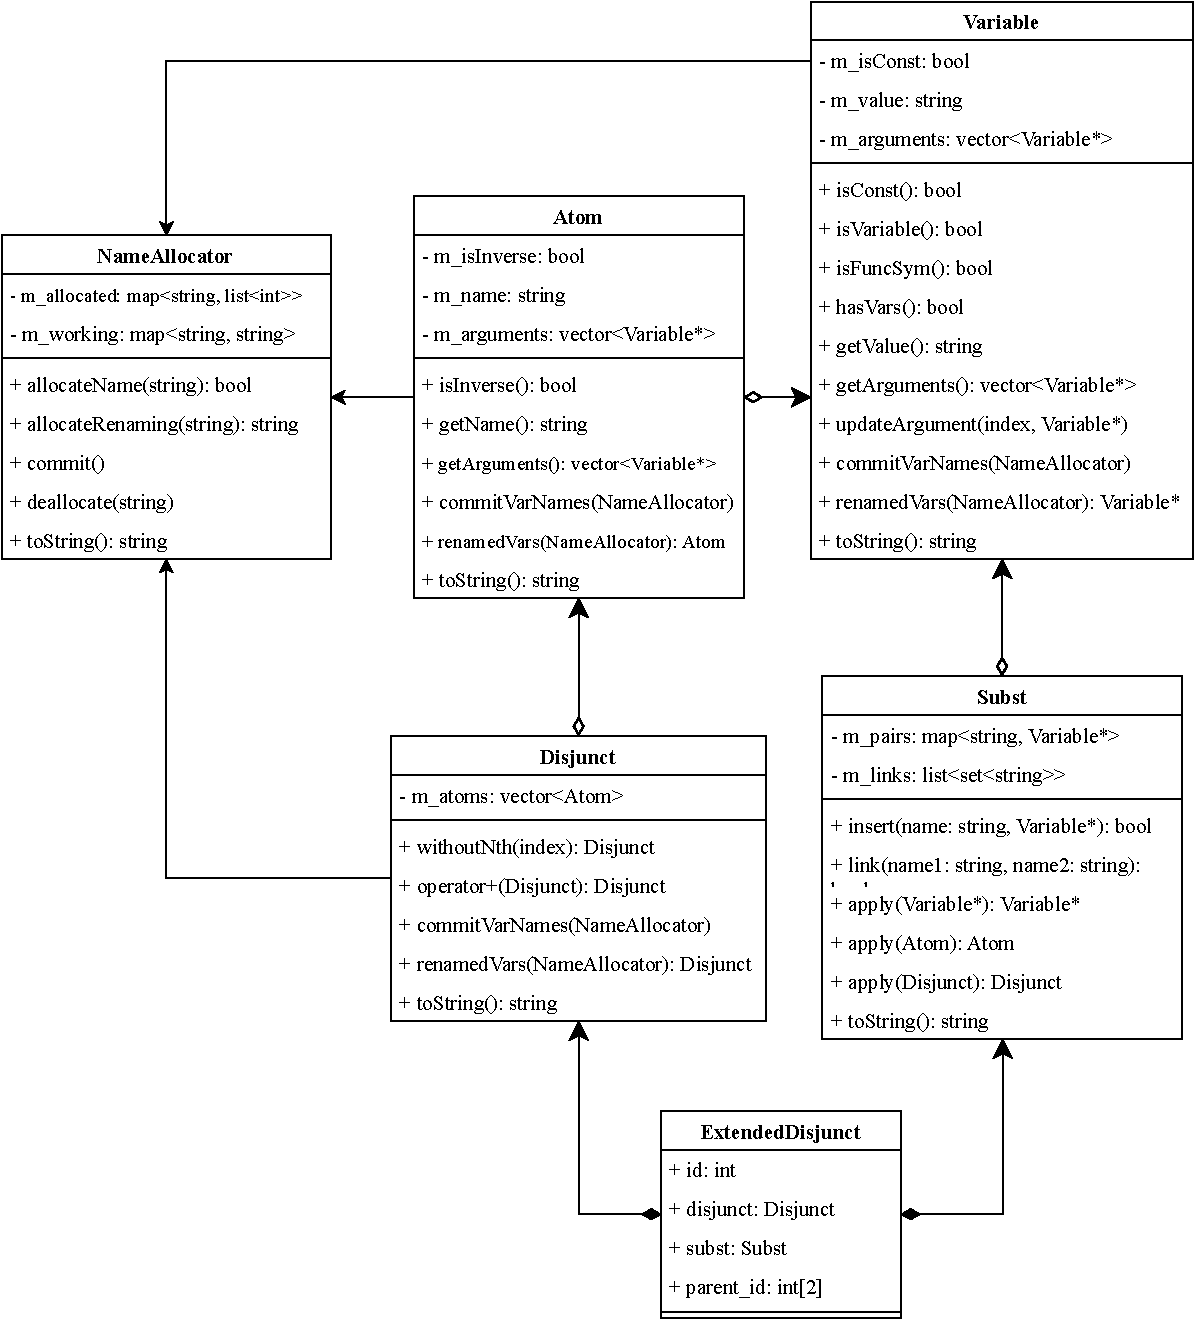
\includegraphics[width=\linewidth]{uml.pdf}
    \caption{Диаграмма классов программы}
\end{figure}

\section{Сборка и запуск ПО}

Для сборки программы используется \texttt{CMake}. Стандартная последовательность команд для сборки и запуска программы:

\begin{verbatim}
mkdir build && cd build && cmake ..
make app && ./app # сборка и запуск программы
make unittests && ./unittests # опциональный запуск юнит-тестов
\end{verbatim}

Альтернативно, можно собрать и запустить программу с помощью \texttt{makefile} скрипта в корневой папке используя цель <<\texttt{app}>>.

Основная программа работает в цикле REPL (read-evaluate-print loop). Сначала нужно выбрать режим работы. Допустимые значения --- \texttt{u} для унификации единичных атомов и \texttt{r} для запуска алгоритма резолюции. В режиме резолюции первой строкой необходимо ввести список аксиом в формате выражений описанных EBNF грамматикой отделяя выражения символом <<\texttt{;}>>. Во второй строке необходимо ввести одно выражение, представляющее цель (не ее отрицание). Пример работы программы:

\begin{verbatim}
repl for resolution method:
select mode (u - unify, r - resolve): u
enter 'end' to exit repl
enter first atom: P(x, f(x))
enter second atom: P(g(y), y)
unified successfully, subst: {x=g(f(...)), y=f(g(...))}
enter first atom: end
select mode (u - unify, r - resolve): r
enter 'end' to exit repl
enter axioms (colon-separated): \forall(x) (P(x) -> Q(x)); P(A)
enter conclusion: Q(A)
1) ~Q(A)
2) ~P(x1) + Q(x1)
3) P(A)
4) ~P(A) (1 + 2) {x1=A}
5)  (3 + 4) {}
resolved: yes
\end{verbatim}

\clearpage

\section{Тестирование ПО}

\subsection{Тестирование унификации двух атомов}

В таблице \ref{tab:unify} представлены тестовые данные для проверки корректности работы алгоритма унификации двух атомов.

\begin{table}[h!]
    \centering
    \caption{Тестовые данные для проверки реализации алгоритма унификации}
    \label{tab:unify}
    \begin{tabular}{|c|c|c|}
        \hline
        Исходные атомы & Подстановка & Описание \\
        \hline
        \hline
        $R(x)$ & $\{x=A\}$ & Успешная \\
        $R(A)$ & & постановка \\
        \hline
        $P(x, f(x, B, g(y)), g(C))$ & $\{x=A,~y=C,$ & Обновление \\
        $P(A, f(A, B, z), g(y))$ & $z=g(C)\}$ & значений переменных \\
        \hline
        $Q(S, x, F, G, y, H)$ & $\emptyset$ & Конфликт связанных \\
        $Q(y, A, F, G, x, H)$ & & переменных \\
        \hline
        $P(x, f(g(x)))$ & $\{x=y=f(g(...))\}$ & Рекурсивная \\
        $P(y, y)$ & & подстановка \\
        \hline
        $H(x, g(z), z, o(x))$ & $\{x=f(g(t(...))),$ & Косвенная \\
        $H(f(y), y, t(x), o(x))$ & $y=g(t(f(...))),$ & рекурсия \\
        & $z=t(f(g(...)))\}$ & в подстановке \\
        \hline 
    \end{tabular}
\end{table}

\subsection{Тестирование алгоритма нахождения резольвенты для двух дизъюнктов}

%В таблице \ref{tab:resolve1} представлены тестовые данные для проверки реализации алгоритма нахождения резольвенты для двух дизъюнктов.

\begin{table}[h!]
    \centering
    \caption{Тестовые данные для проверки алгоритма поиска резольвенты}
    \label{tab:resolve1}
    \begin{tabular}{|c|c|c|}
        \hline
        Пара дизъюнктов & Резольвента & подстановка \\
        \hline
        \hline
        $A,~~\neg A + B$ & $B$ & $\emptyset$ \\
        \hline
        $\neg A + P(f_0),~~Q(x) + \neg P(x)$ & $\neg A + Q(f_0)$ & $\{x=f_0\}$ \\
        \hline
        $\neg P(x, y) + \neg P(y, z) + P(x, z)$ & $\neg P(3, y) + \neg P(y, 5)$ & $\{x=3,$ \\
        $\neg P(3, 5)$ & & $z=5\}$ \\
        \hline
    \end{tabular}
\end{table}

\subsection{Тестирование алгоритма резолюции}

Сценарии тестирования алгоритма резолюции представлены в таблице \ref{tab:resolve}.

\begin{table}[h!]
    \centering
    \caption{Сценарии тестирования алгоритма резолюции}
    \label{tab:resolve}
    \begin{tabular}{|c|l|}
        \hline
        Номер & Исходная задача \\
        \hline
        \hline
        1 & Аксиомы: \\
        & $\forall x \forall y \forall z (Len(x, y) \rightarrow Len(c(z, x), s(y)))$ \\
        & $Len(Nil, 0)$ \\
        & Цель: $\exists x Len(x, s(s(0)))$ \\
        \hline
        & Цепочка вывода \\
        & Аксиомы: $\neg Len(x, y) + Len(c(z, x), s(y)), Len(Nil, 0)$ \\
        & Отрицание цели: $\neg Len(x, s(s(0)))$ \\
        & 1) $\neg Len(x, s(s(0)))$ \\
        & 2) $\neg Len(x_1, y_1) + Len(c(z_1, x_1), s(y_1))$ \\
        & 3) $Len(Nil, 0)$ \\
        & 4) $\neg Len(x_2, s(0))~~(1+2)~~\{x=c(z_1, x_1), y_1=s(0)\}$ \\
        & 5) $Len(c(z_2, Nil), s(0))~~(2+3)~~\{x_1=Nil, y_1=0\}$ \\
        & 6) $\square~~(4+5)~~\{x_2=c(z_2, Nil)\}$ \\
        \hline
        \hline
        2 & Аксиомы: \\
        & $\forall x (S(x) + M(x))$ \\
        & $\neg \exists x (M(x) \& L(x, Lena))$ \\
        & $\forall x (S(x) \rightarrow L(x, Snow))$ \\
        & $\forall y (L(Lena, y) = \neg L(Petya, y))$ \\
        & $L(Petya, Rain)$ \\
        & $L(Petya, Snow)$ \\
        & Цель: $\exists x (M(x) \& \neg S(x))$ \\
        \hline
        & Цепочка вывода \\
        & Аксиомы: $S(x) + M(x), \neg M(x_2) + \neg L(x_2, Lena),$ \\
        & $\neg S(x_2) + L(x_2, Snow), \neg L(Lena, y) + \neg L(Petya, y),$ \\
        & $L(Petya, y) + L(Lena, y), L(Petya, Rain), L(Petya, Snow)$ \\
        & Отрицание цели: $\neg M(x) + S(x)$ \\
        & 1) $\neg M(x) + S(x)$ \\
        & 2) $S(x_1) + M(x_1)$ \\
        & 3) $\neg S(x_4) + L(x_4, Snow)$ \\
        & 4) $\neg L(Lena, y_1) + \neg L(Petya, y_1)$ \\
        & 5) $L(Petya, Snow)$ \\
        & 6) $\neg M(x_6) + L(x_6, Snow)~~(1 + 3)~~\{x=x_4\}$ \\
        & 7) $M(x_7) + L(x_7, Snow)~~(2 + 3)~~\{x_1=x_4\}$ \\
        & 8) $\neg L(Lena, Snow)~~(4 + 5)~~\{y_1=Snow\}$ \\
        & 9) $\neg M(Lena)~~(6 + 8)~~\{x_6=Lena\}$ \\
        & 10)$M(Lena)~~(7 + 8)~~\{x_7=Lena\}$ \\
        & 11)$\square~~(9 + 10)~~\{\}$ \\
        \hline
    \end{tabular}
\end{table}
